\chapter{A LabVIEW program}

A feladat megvalósításához a Queued Message Handler Template-t választottam.
Ez a tervezési minta segített a hatékonyabb és strukturáltabb kódírásban.
Az állapotgép felépítése ennek segítségével jelentősen egyszerűbb, mint
ha azt a nulláról kellett volna létrehozni.

\section{Az állapotgép felépítése}

A lehetséges állapotok:
\newcommand{\alma}[1]{\item \texttt{#1}}
\begin{enumerate}
  \alma{Initialize} -- program indításakor
  \alma{Reinit Values} -- indításkor és kilépéskor
  \alma{Update Display} -- üzenet kiíratásakor
  \alma{Open Settings} -- settings gomb megnyomásakor
  \alma{Save Settings} -- ok gomb megnyomásakor
  \alma{Get About} -- start gomb megnyomásakor
  \alma{Set About} -- \texttt{Get About} után
  \alma{Get Data} -- dátum változtatáskor
  \alma{Set Detailed} -- \texttt{Get Data} után
  \alma{Set Panel} -- \texttt{Get Data} után, vagy inverter változtatásakor
  \alma{Error} -- error esetén
  \alma{Exit} -- stop gomb megnyomásakor
\end{enumerate}

\section{Az érkező adatok fogadása}

Az általam létrehozott API az adatokat JSON formátumban továbbította a
külvilág számára. Ezeket az objektumokat a JSON text tools segítségével
alakítottam cluster-ekké vagy tömbökké attól függően, hogy a JSON egy
\texttt{object} vagy egy \texttt{array} volt.

\subsection{Általános adatok}

Az \texttt{`/about`} útvonal által szolgáltatott adatok, azok typescript
típusa, illetve LabVIEW-ban lévő konstans közötti megfeleltetést a
\ref{fig:about}. ábra tartalmazza.
\begin{figure}[H]
  \centering
  \begin{minipage}{.3\textwidth}
    \begin{minted}{json}
{
  "dates": [ 
    "2023-05-24"
  ],
  "count": {
    "inverter": 8,
    "panel": 4
  }
}
    \end{minted}
  \end{minipage}\begin{minipage}{.3\textwidth}
    \begin{minted}{typescript}
type About = {
  dates: Array<DateString>;
  count: {
    inverter: number;
    panel: number;
  };
};
    \end{minted}
  \end{minipage}\begin{minipage}{.3\textwidth}
    \flushright
    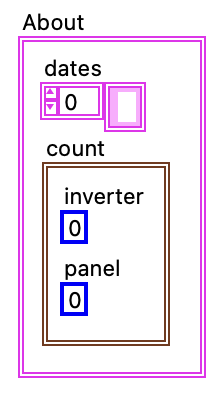
\includegraphics[height=5cm]{static/lv-about.png}
  \end{minipage}

  \caption{Az általános adatok közötti megfeleltetés}
  \label{fig:about}
\end{figure}

\subsection{Panel adatok}

A \texttt{`/panel/:date`} útvonal által szolgáltatott adatok, azok typescript
típusa, illetve LabVIEW-ban lévő konstans közötti megfeleltetést a
\ref{fig:panel}. ábra tartalmazza.
\begin{figure}[H]
  \centering
  \begin{minipage}{.3\textwidth}
    \begin{minted}{json}
[
  3011, // panel 01
  3047, // panel 02
  // ..... panel ..
  2595  // panel 32
]
    \end{minted}
  \end{minipage}\begin{minipage}{.3\textwidth}
    \begin{minted}{typescript}
type Panel = Array<number>;
    \end{minted}
  \end{minipage}\begin{minipage}{.3\textwidth}
    \flushright
    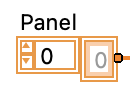
\includegraphics[height=2cm]{static/lv-panel.png}
  \end{minipage}

  \caption{A panel adatok közötti megfeleltetés}
  \label{fig:panel}
\end{figure}

\subsection{Részletes adatok}

A \texttt{`/detailed/:date`} útvonal által szolgáltatott adatok, azok typescript
típusa, illetve Lab\-VIEW-ban lévő konstans közötti megfeleltetést a
\ref{fig:detailed}. ábra tartalmazza.
\begin{figure}[H]
  \centering
  \begin{minipage}{.3\textwidth}
    \begin{minted}{json}
{
  "power": [
    0,
    // ...
  ],
  "sum": [
    0,
    // ...
  ],
  "hour": [
    "00:00",
    // ...
  ]
}
    \end{minted}
  \end{minipage}\begin{minipage}{.3\textwidth}
    \begin{minted}{typescript}
type Detailed = {
  power: Array<number>;
  sum: Array<number>;
  hour: Array<string>;
}:
    \end{minted}
  \end{minipage}\begin{minipage}{.3\textwidth}
    \flushright
    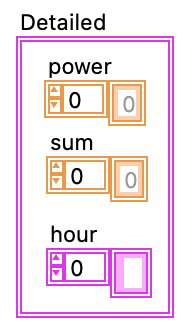
\includegraphics[height=6cm]{static/lv-detailed.png}
  \end{minipage}

  \caption{A részletes adatok közötti megfeleltetés}
  \label{fig:detailed}
\end{figure}

\section{Az adatok megjelenítése és feldolgozása}

A beérkezett adatok alapján a program front panel-je dinamikusan változik.
A részletes adatokat (negyedórás teljesítmény és energia adatok) gráfokon
jelenítettem meg, melyet a \ref{fig:graphs} ábra szemléltet.

\begin{figure}[ht]
  \centering
  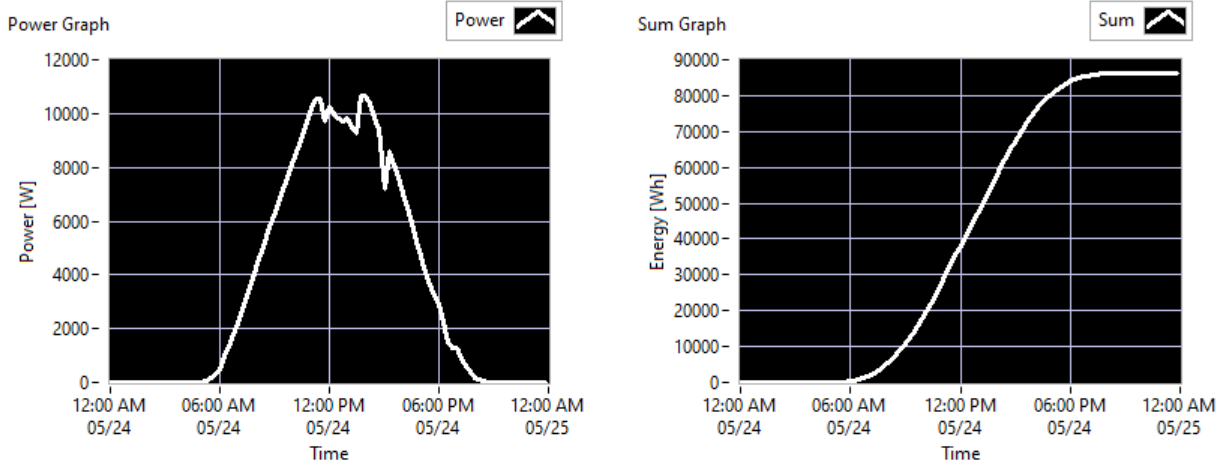
\includegraphics[width=.7\textwidth]{static/windows-graph.png}
  \caption{A részletes adatok grafikus megjelenítése}
  \label{fig:graphs}
\end{figure}

A panelenkénti termelési adatokat inverterenként összegeztem, valamint
megjelenítettem azt is, hogy egymáshoz képest milyen volt a relatív
teljesítményük.

\begin{figure}[ht]
  \centering
  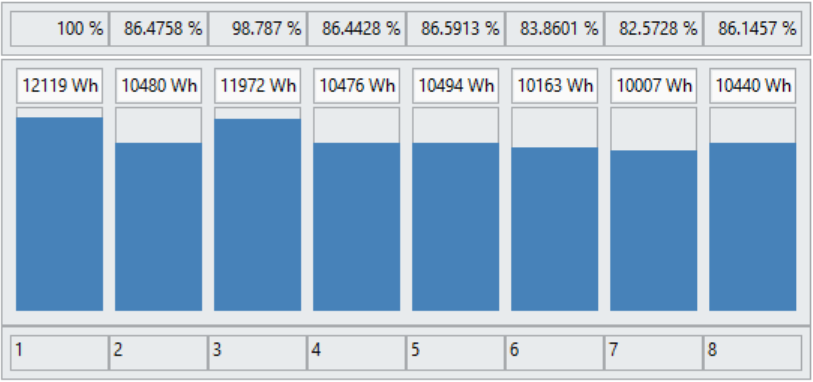
\includegraphics[height=.3\textwidth]{static/windows-inverter-energy.png}
  \caption{Az inverterenkénti energia adatok}
  \label{fig:inverter-energy}
\end{figure}

Megjelenítettem továbbá egy választható inverterhez tartozó panelok
termelési adatait, valamint relatív teljesítményüket.

\begin{figure}[ht]
  \centering
  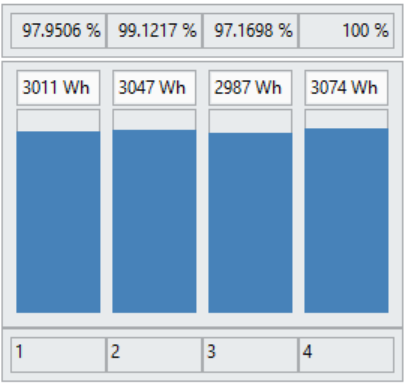
\includegraphics[height=.3\textwidth]{static/windows-panel-energy.png}
  \caption{Tetszőleges inverterhez tartozó panelok termelése}
  \label{fig:panel-energy}
\end{figure}

Azt hogy melyik naphoz, és melyik inverterhez tartozó adatokat szeretnénk
megtekinteni, egy-egy ring segítségével választhatjuk meg.
\begin{figure}[ht]
  \centering
  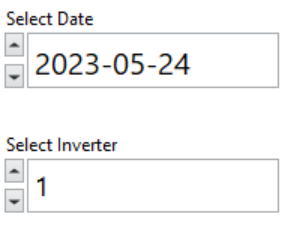
\includegraphics[height=.2\textwidth]{static/windows-ring.png}
  \caption{Tetszőleges inverterhez tartozó panelok termelése}
  \label{fig:ring}
\end{figure}

A program teljes front panel-je megtekinthető a \ref{fig:fp}. ábrán.
\begin{figure}[H]
  \centering
  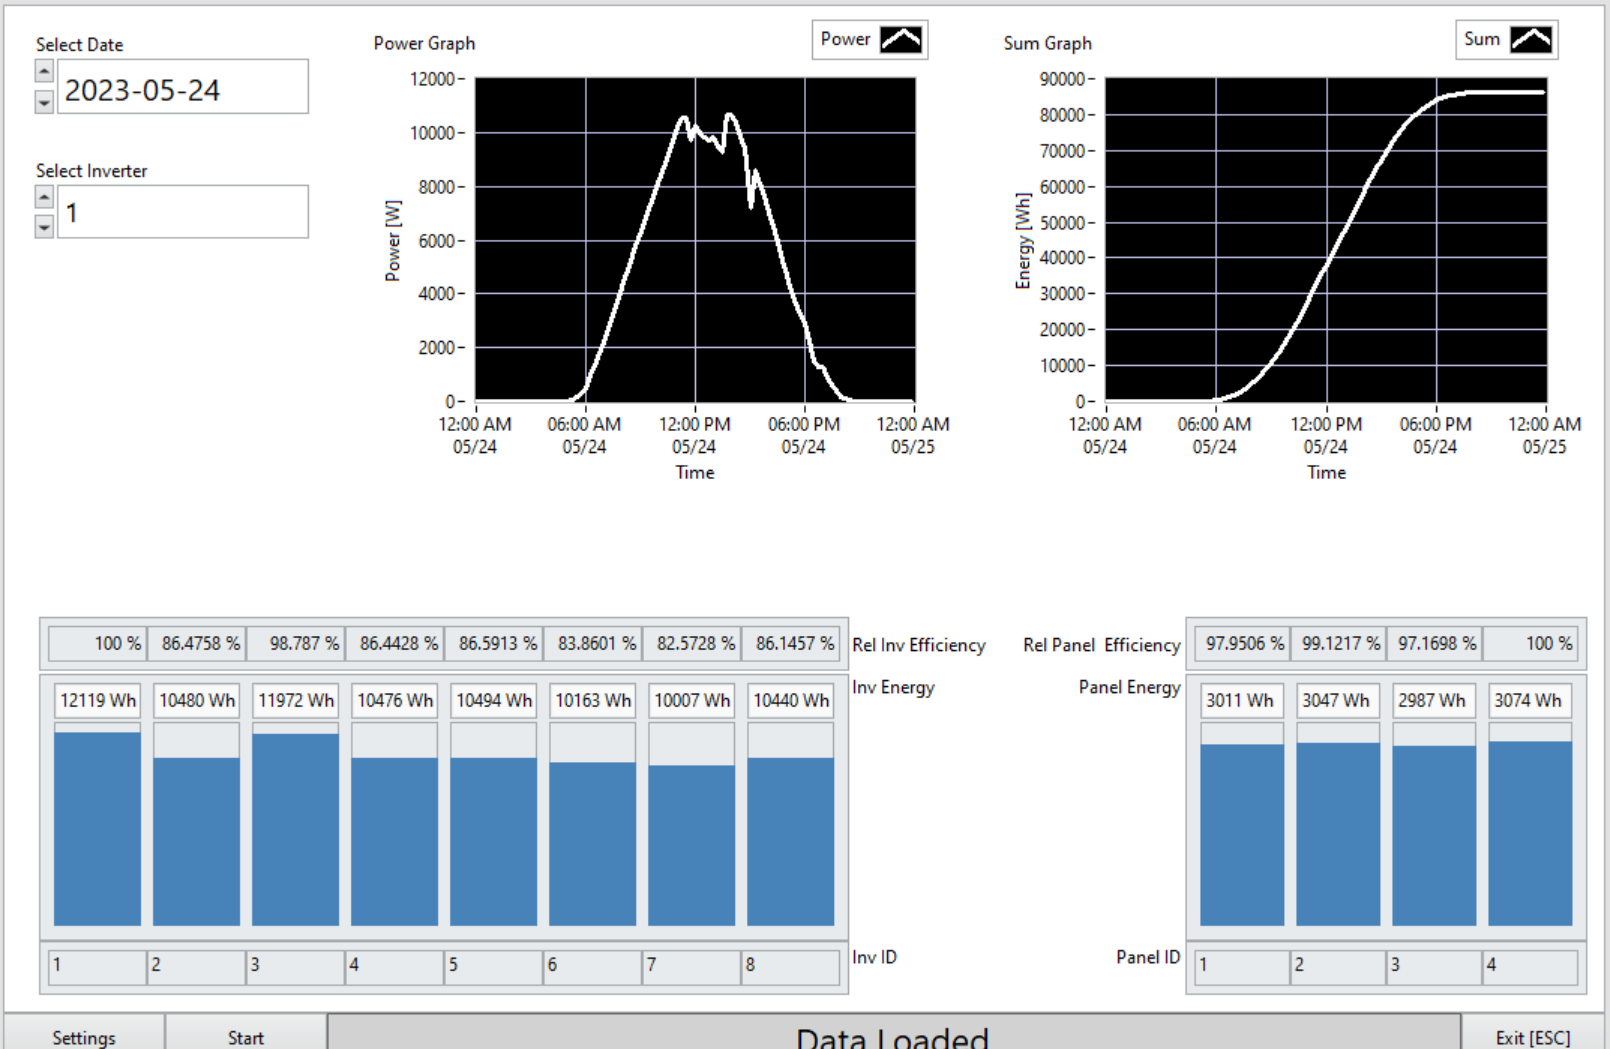
\includegraphics[width=\textwidth]{static/windows-fp.png}
  \caption{A program teljes front panel-je}
  \label{fig:fp}
\end{figure}
